\chapter{Intercambio de Correo Seguro OpenPGP}

\section{Descripción del escenario}

Para poder enviar un mensaje \textbf{cifrado} a alguien, es imprescindible disponer de su \textbf{clave pública}. El intercambio de claves se realiza enviando primero la propia clave pública al compañero (adjunta en un correo), y a su vez recibiendo la del compañero. Una vez ambas partes disponen de las claves públicas del otro, es posible enviar mensajes cifrados y firmados.

El esquema del intercambio es:

\begin{center}
    \textbf{Nicolás} $\xrightarrow{\text{mi\_clave\_publica.asc + firmado}}$ \textbf{Wafa} \\[6pt]
    \textbf{Wafa} $\xrightarrow{\text{mi\_clave\_publica.asc + firmado}}$ \textbf{Nicolás} \\[6pt]
    \textbf{Nicolás} $\xrightarrow{\text{Firmado + Cifrado con clave de Wafa}}$ \textbf{Wafa} \\[6pt]
    \textbf{Wafa} $\xrightarrow{\text{Firmado + Cifrado con clave de Nicolás}}$ \textbf{Nicolás}
\end{center}

\section{Paso 1 -- Envío de nuestra clave pública}

Se compone un mensaje dirigido a Wafa Azdad Triki (\texttt{azdadwafa0@gmail.com}) con asunto \textit{``Esta es mi clave publica y mi correo firmado''}. Se adjunta manualmente el fichero \texttt{.asc} de nuestra clave pública exportada desde el \textit{OpenPGP Key Manager} de Thunderbird, y se activa la \textbf{firma digital} para que Wafa pueda también importar nuestra clave directamente del mensaje firmado.

\begin{figure}[H]
    \centering
    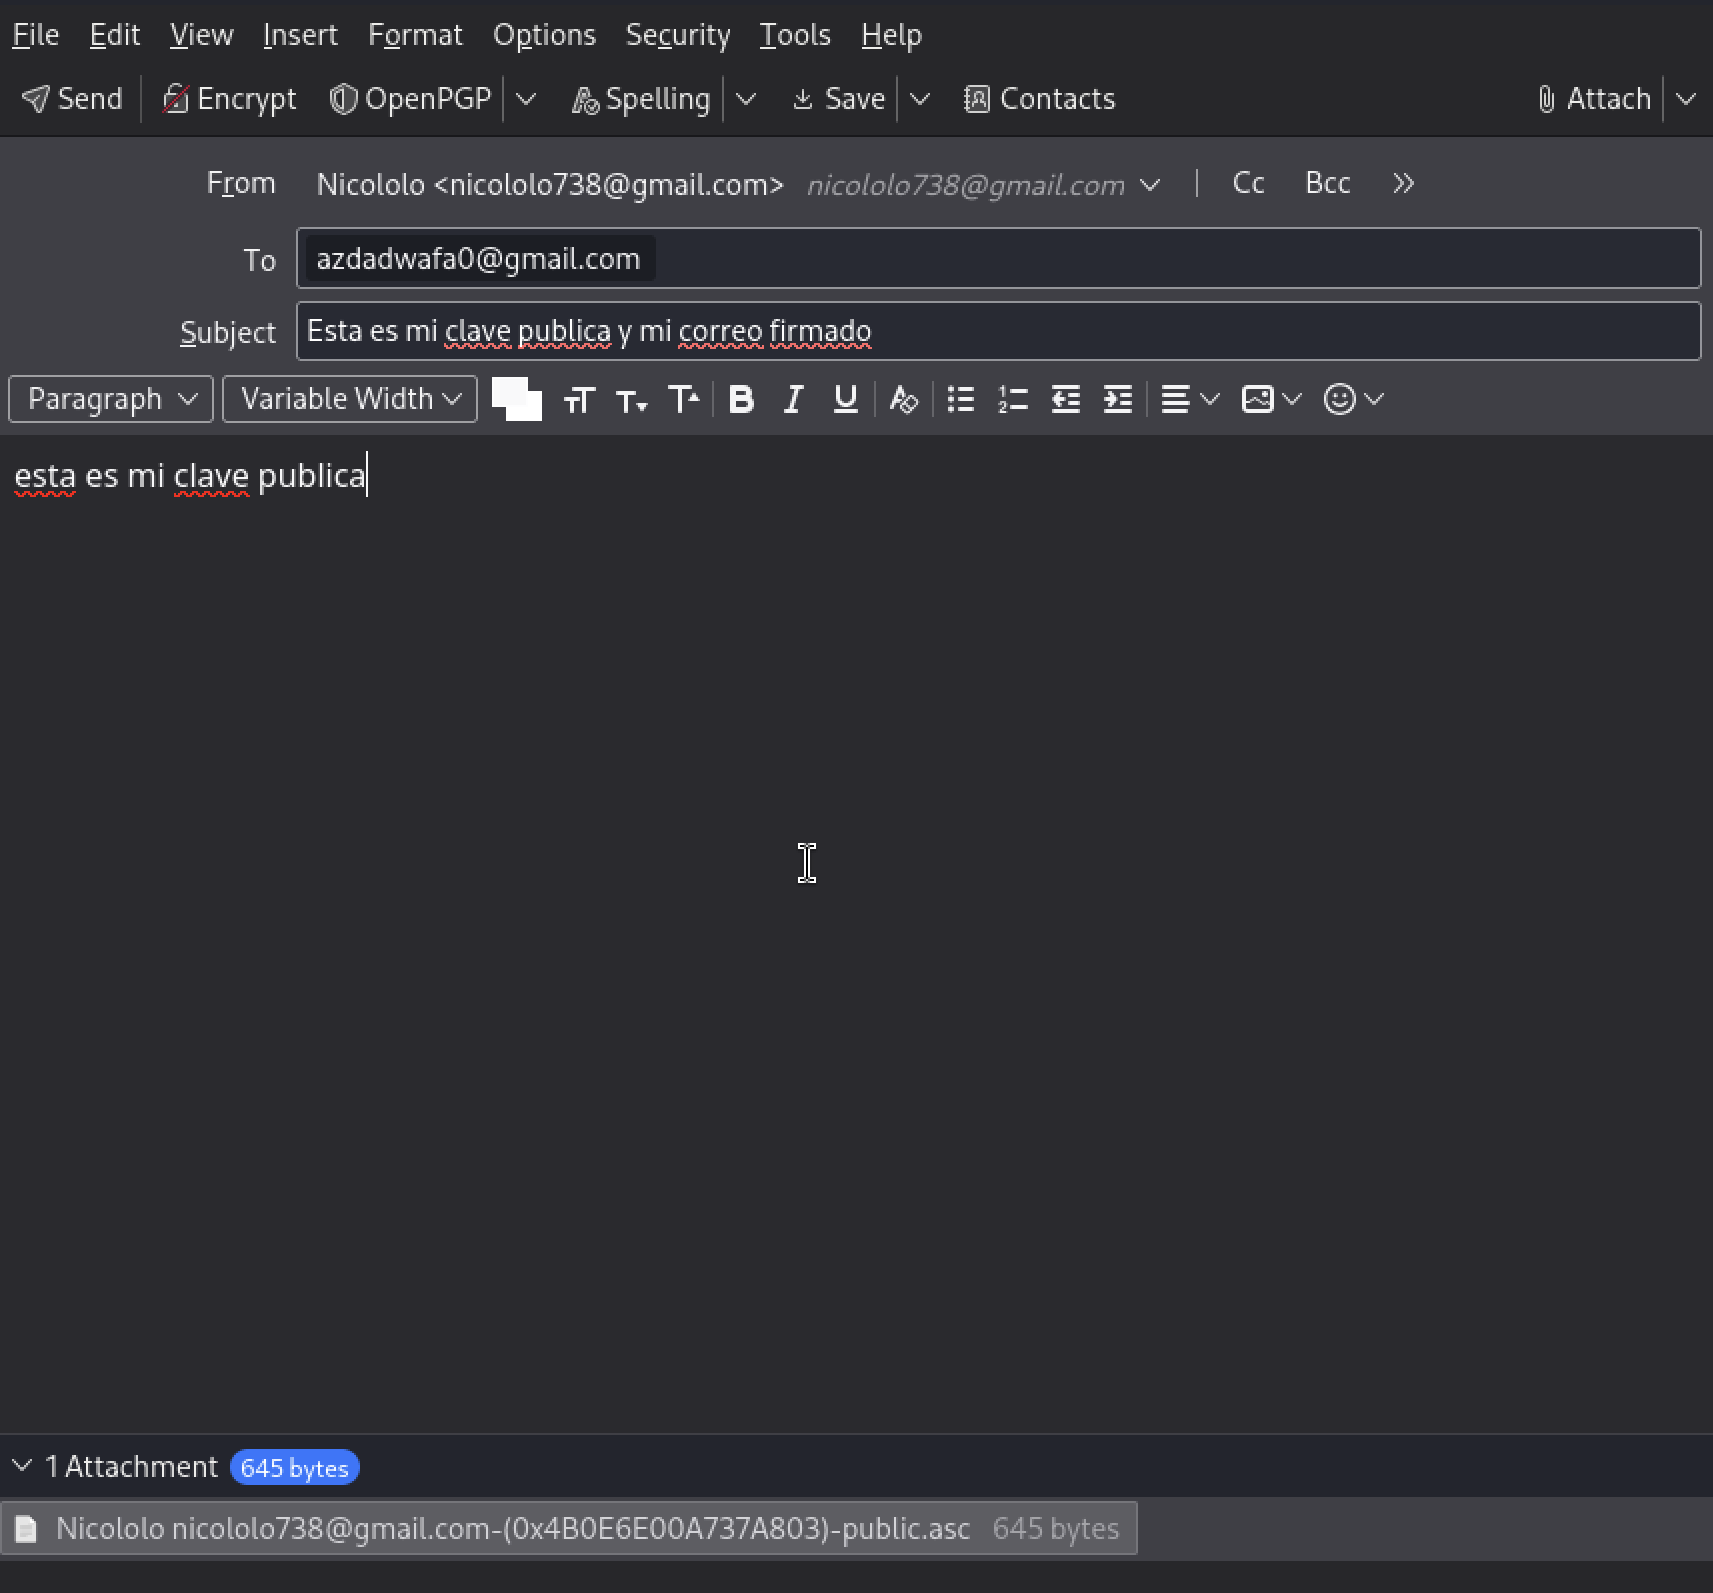
\includegraphics[width=\textwidth]{Imagenes/5-EnviodecorreoClavePublica.png}
    \caption{Composición del mensaje con nuestra clave pública adjunta y firma activa}
    \label{fig:envio_clave_publica}
\end{figure}

El fichero adjunto es \texttt{Nicololo nicololo738@gmail.com-(0x4B0E6E00A737A803)-public.asc} (645\,bytes), que contiene únicamente la parte pública de nuestra clave OpenPGP.

\section{Paso 2 -- Recepción de la clave pública de la compañera}

Wafa nos envía su clave pública OpenPGP en un correo con asunto \textit{``Mi clave publica OpenPGP''} (recibido a las 16:56 del 5 de marzo de 2026). El correo aparece marcado como \textbf{OpenPGP} en Thunderbird. El adjunto es \texttt{mi\_clave\_publica.asc} (3,1\,KB), que contiene su clave pública RSA\,4096.

\begin{figure}[H]
    \centering
    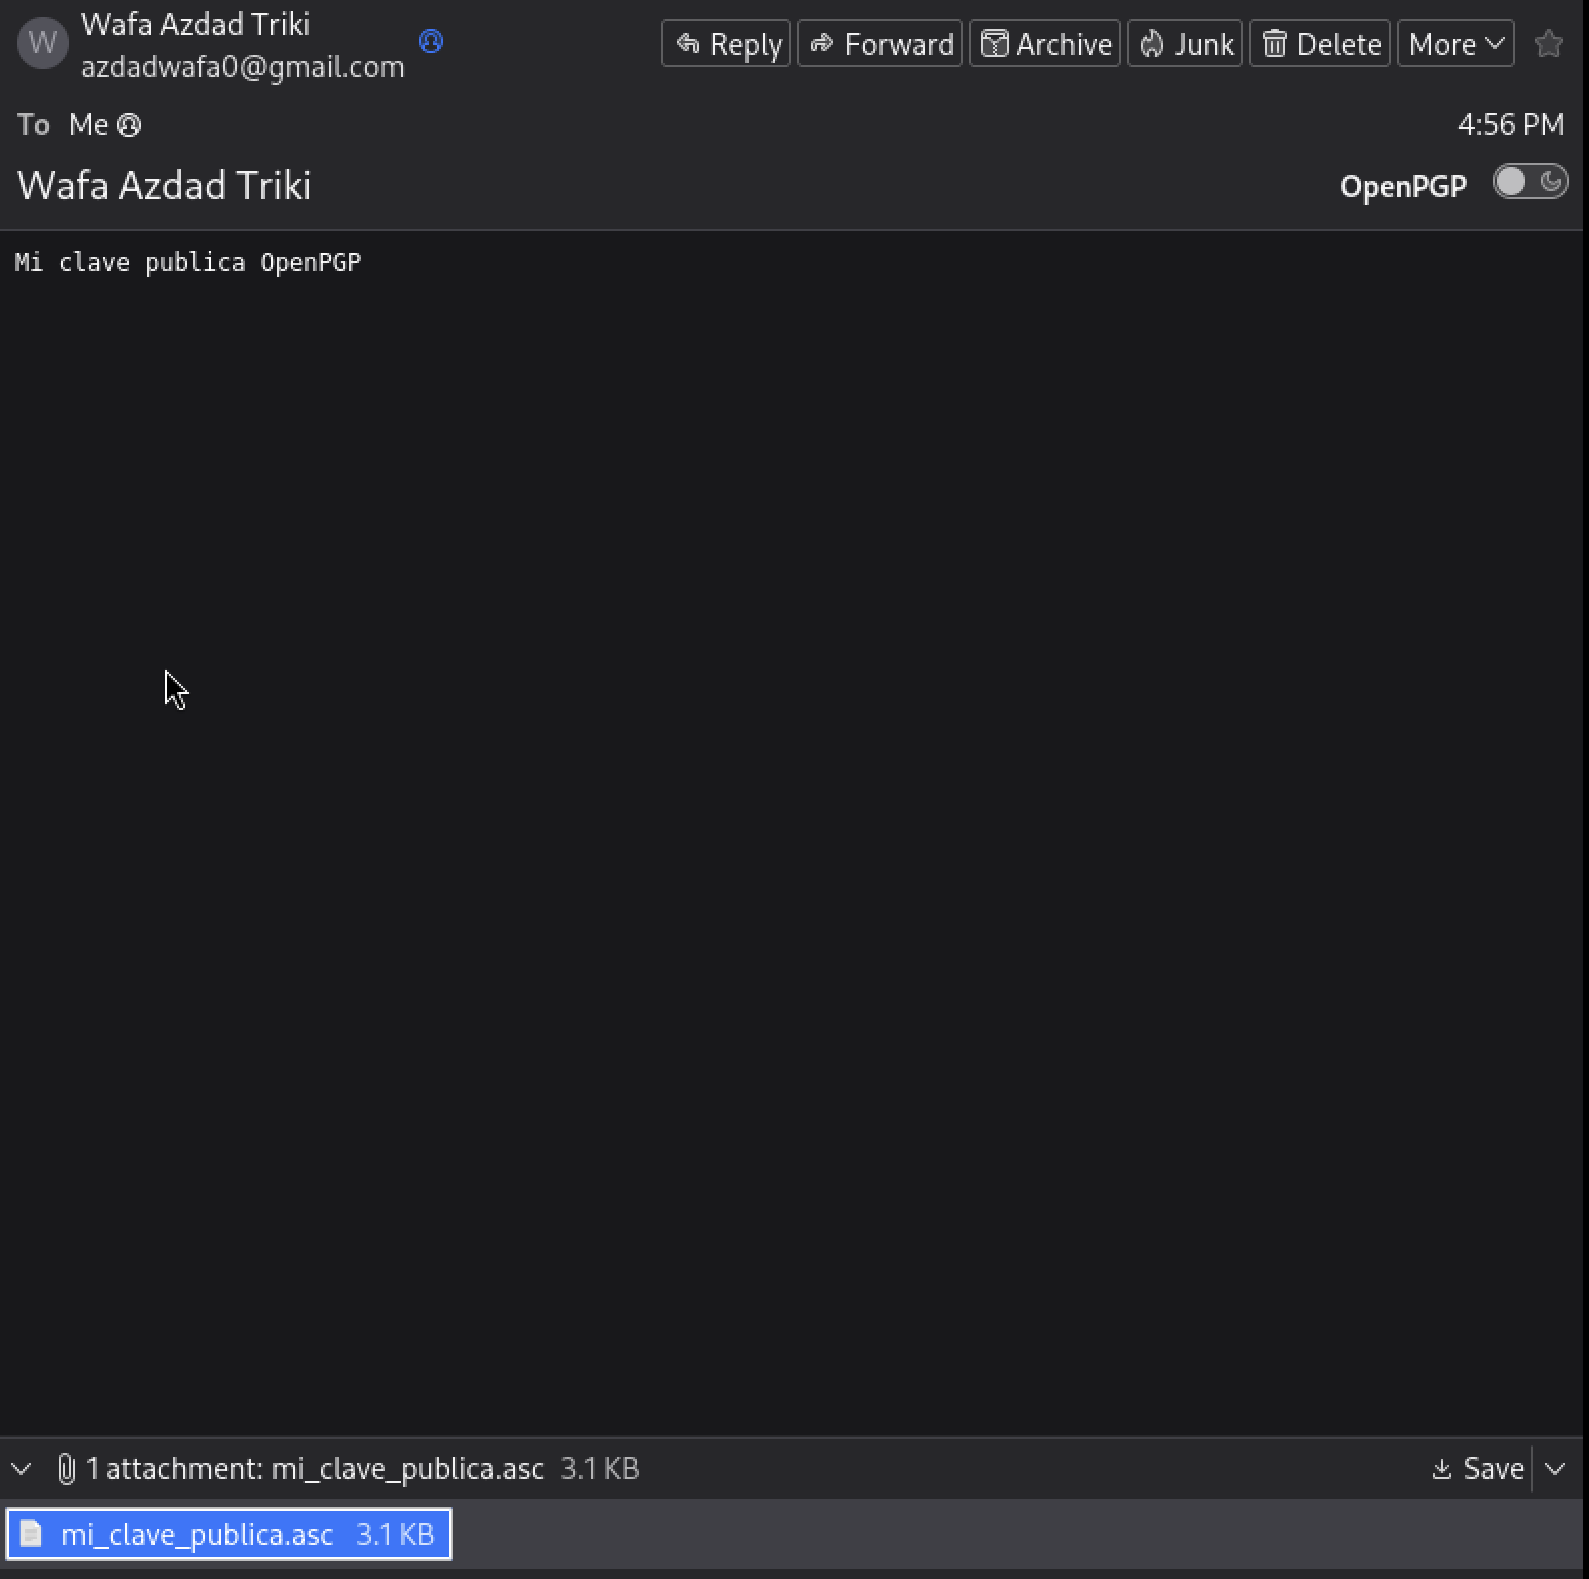
\includegraphics[width=\textwidth]{Imagenes/6-ClavePublicaWafa.png}
    \caption{Correo recibido de Wafa Azdad Triki con su clave pública OpenPGP adjunta}
    \label{fig:clave_publica_wafa}
\end{figure}

Se importa la clave de Wafa en Thunderbird a través del \textit{OpenPGP Key Manager} $\rightarrow$ \textit{Import Public Key(s) from File}. Su Key ID es \texttt{0x62C2D55D111C2F3C}.

\subsection{Corrección puntual:}
Como se puede observar en la imagen, mi compañera Wafa ha incluido en el 
mensaje un adjunto con su clave pública, pero no ha firmado digitalmente el 
correo. Esto supone una desviación del guión original de la práctica aunque el 
resto de los pasos se mantienen intactos. Para suplir este punto 
instalé thunderbird en el sistema anfitrión y me envié un correo a modo de
corrección para que se observé el comportamiento de que debiese haberse visto.

\begin{figure}[H]
    \centering
    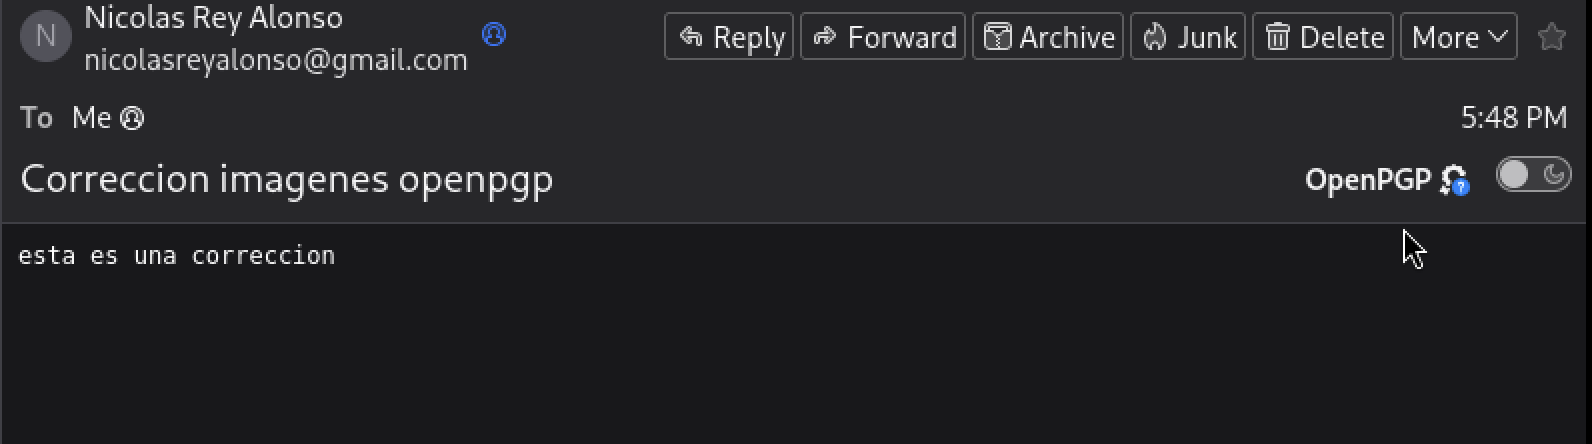
\includegraphics[width=\textwidth]{Imagenes/6.2.png}
    \caption{Correo recibido de mi mismo firmado}
    \label{fig:clave_publica_yo}
\end{figure}


\section{Paso 3 -- Envío de mensaje cifrado y firmado}

Una vez que disponemos de la clave pública de Wafa, componemos el mensaje cifrado y firmado. En la ventana de composición se observa los botones \textbf{Encrypt} y \textbf{OpenPGP} en la barra de herramientas. El mensaje de ejemplo tiene asunto \textit{``Ahora encriptado con tu clave''} y cuerpo \textit{``hola wafa''}.

\begin{figure}[H]
    \centering
    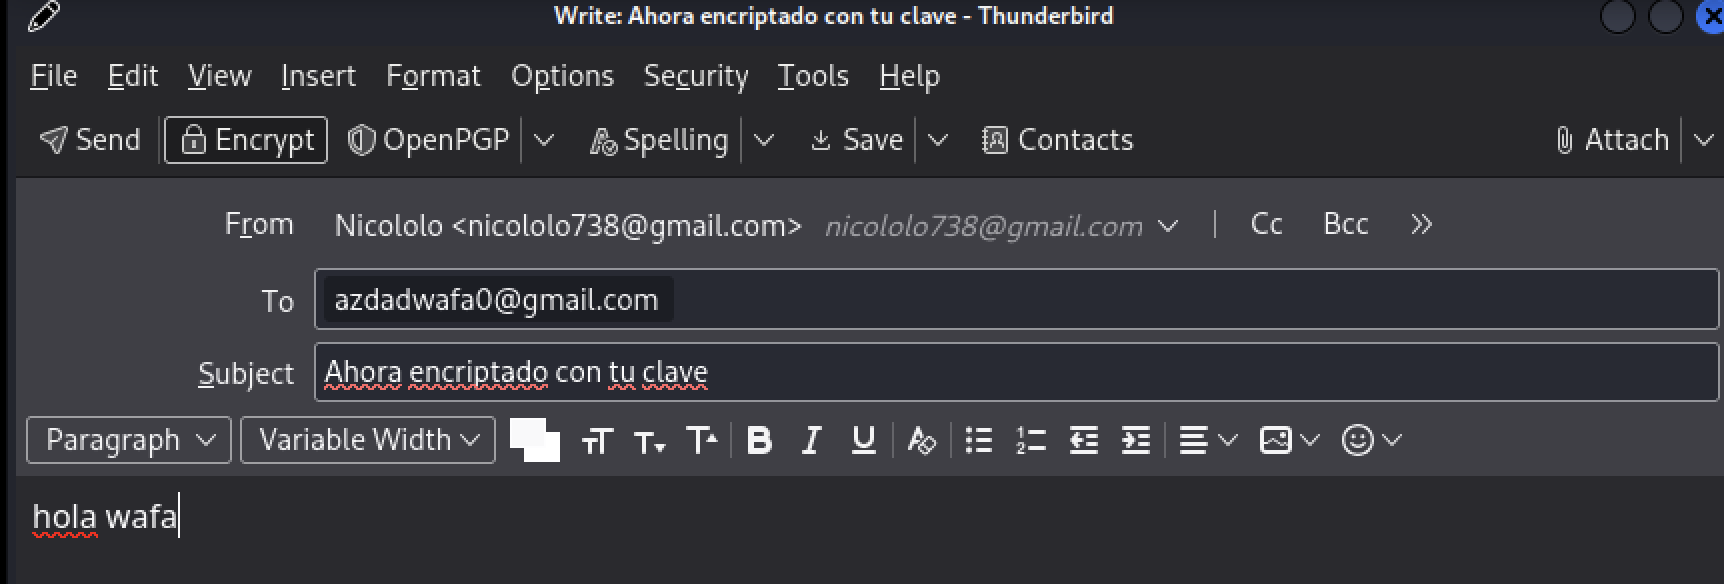
\includegraphics[width=\textwidth]{Imagenes/7-EnvioCorreoEncriptado.png}
    \caption{Composición del mensaje cifrado y firmado con OpenPGP dirigido a Wafa}
    \label{fig:envio_cifrado_firmado}
\end{figure}

\subsection{Opciones de seguridad OpenPGP activas}

Desplegando el menú \textbf{OpenPGP} de la barra de herramientas se puede verificar que las opciones activas son:

\begin{itemize}[label=\textbullet]
    \item \textbf{OpenPGP} (marcado): se usa el estándar OpenPGP, no S/MIME.
    \item \textbf{Encrypt} (marcado): el cuerpo del mensaje se cifrará con la clave pública de Wafa.
    \item \textbf{Encrypt Subject} (marcado): el asunto también se cifra.
    \item \textbf{Digitally Sign} (marcado): el mensaje se firma digitalmente con nuestra clave privada.
\end{itemize}

\begin{figure}[H]
    \centering
    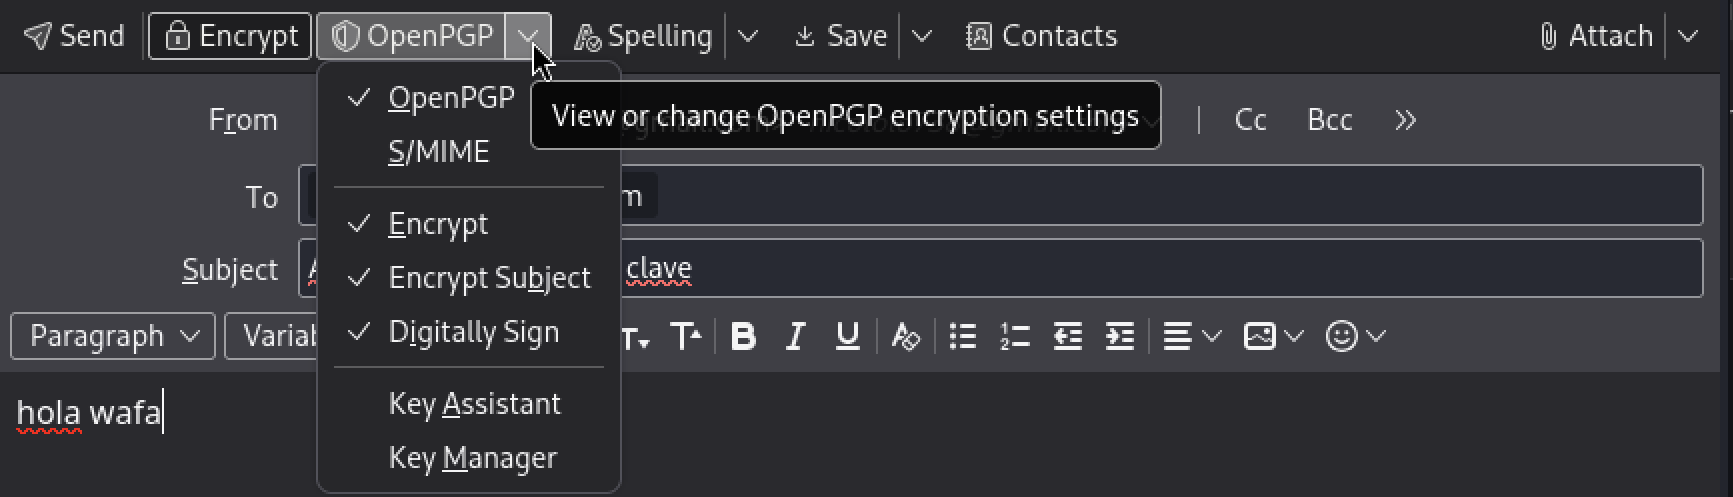
\includegraphics[width=0.75\textwidth]{Imagenes/8-OpcionesEnvioEncriptadoOpenPGP.png}
    \caption{Menú OpenPGP mostrando las opciones de cifrado y firma activas}
    \label{fig:opciones_openpgp}
\end{figure}

\section{Paso 4 -- Recepción del mensaje cifrado y firmado de la compañera}

Se recibe el mensaje cifrado y firmado de Wafa Azdad Triki (5 de marzo de 2026, 17:05). Thunderbird lo descifra automáticamente usando nuestra clave privada y muestra el cuerpo \textit{``Firmado y cifrado''}. En la esquina superior derecha aparece el indicador \textbf{OpenPGP} con iconos de candado y firma.

\begin{figure}[H]
    \centering
    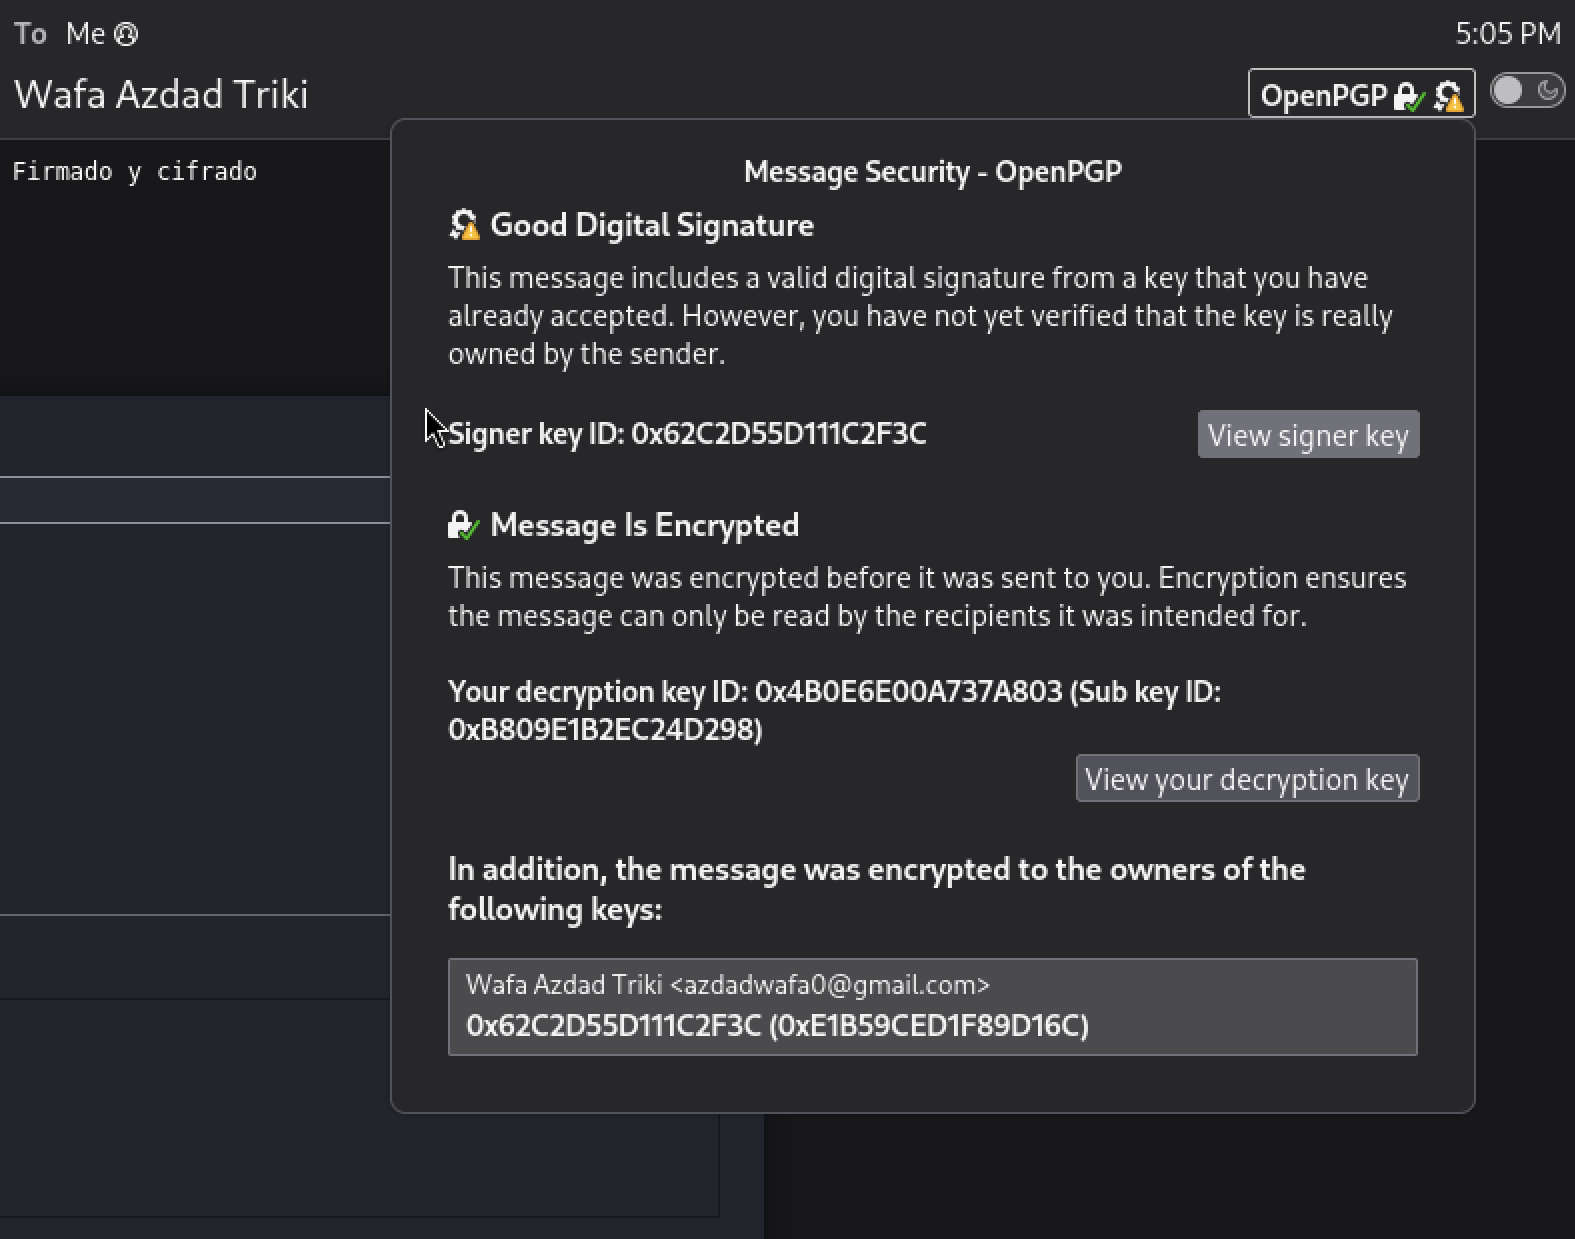
\includegraphics[width=\textwidth]{Imagenes/9-SelloAmarilloPrevioAAceptarMaximaConfianza.png}
    \caption{Mensaje cifrado y firmado de Wafa recibido en la bandeja de entrada de Thunderbird con sello amarillo}
    \label{fig:mensaje_recibido}
\end{figure}

El mensaje lleva el adjunto \texttt{OpenPGP\_0x62C2D55D111C2F3C.asc} (3,1\,KB), que es la clave pública de Wafa incluida automáticamente por Thunderbird.

La firma aparece con sello amarillo porque aún no se ha conferido \textbf{confianza explícita} a la clave de Wafa.

\subsection{Verificación de la seguridad del mensaje en Thunderbird}

Al pulsar sobre el indicador \textbf{OpenPGP} en la cabecera del mensaje se abre el panel de seguridad \textbf{Message Security -- OpenPGP}, que muestra:

\begin{itemize}[label=\textbullet]
    \item \textbf{Good Digital Signature}: la firma es válida. Sin embargo, indica que ``you have not yet verified that the key is really owned by the sender'' porque aún no se ha asignado confianza a la clave de Wafa.
    \item \textbf{Signer key ID}: \texttt{0x62C2D55D111C2F3C} (clave maestra de Wafa).
    \item \textbf{Message Is Encrypted}: el mensaje estaba cifrado antes de ser enviado.
    \item \textbf{Your decryption key ID}: \texttt{0x4B0E6E00A737A803} (nuestra clave), subclave \texttt{0xB809E1B2EC24D298}.
    \item El mensaje también estaba cifrado para los propietarios de la clave \texttt{0x62C2D55D111C2F3C} de Wafa (encriptado para ambos interlocutores).
\end{itemize}

\begin{figure}[H]
    \centering
    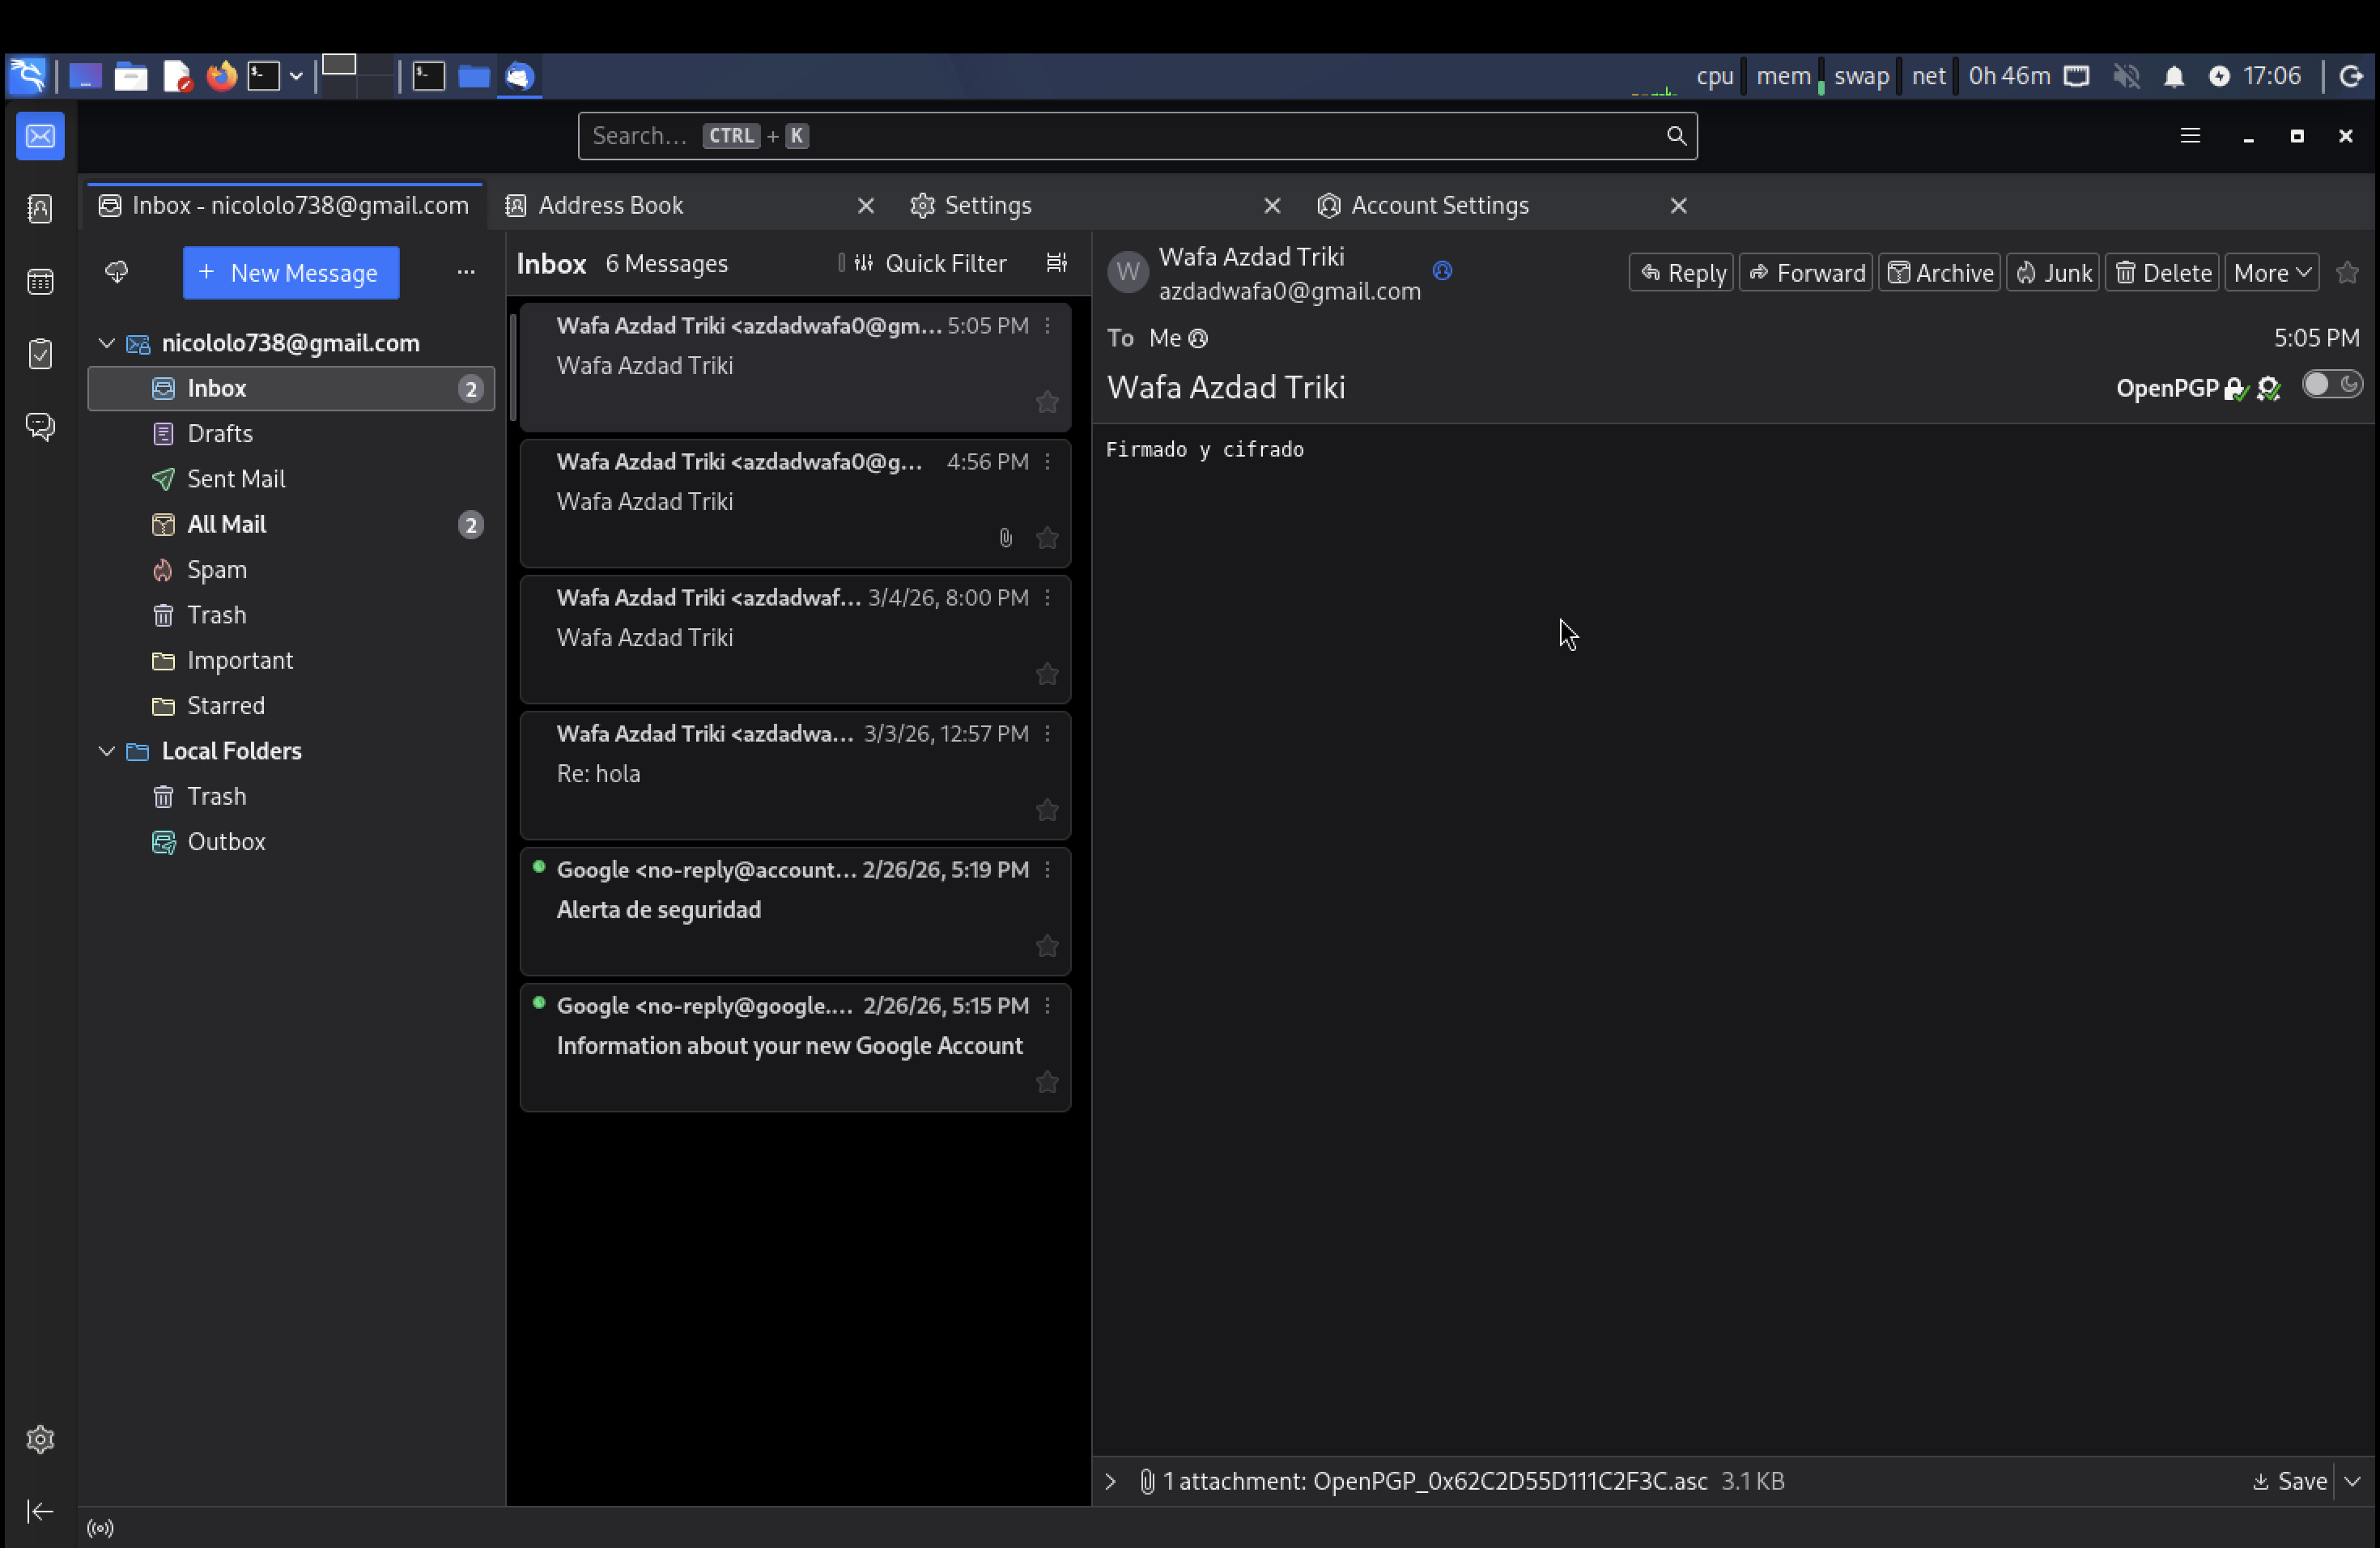
\includegraphics[width=0.75\textwidth]{Imagenes/10-SelloVerdePostAceptarMaximaConfianza.png}
    \caption{Panel de seguridad del mensaje mostrando firma válida y cifrado correcto con sello verde tras conceder la maxima confianza}
    \label{fig:seguridad_mensaje}
\end{figure}

